\documentclass[a4paper]{article}

\usepackage{INTERSPEECH2016}

\usepackage{graphicx}
\usepackage{amssymb,amsmath,bm}
\usepackage{textcomp}
\usepackage{verbatim}
\usepackage{cite}
\usepackage{upgreek}

\def\vec#1{\ensuremath{\bm{{#1}}}}
\def\mat#1{\vec{#1}}


\sloppy % better line breaks
\ninept

\title{Entropy-based segmentation of birdcalls using Fourier transform phase}

%%%%%%%%%%%%%%%%%%%%%%%%%%%%%%%%%%%%%%%%%%%%%%%%%%%%%%%%%%%%%%%%%%%%%%%%%%
%% If multiple authors, uncomment and edit the lines shown below.       %%
%% Note that each line must be emphasized {\em } by itself.             %%
%% (by Stephen Martucci, author of spconf.sty).                         %%
%%%%%%%%%%%%%%%%%%%%%%%%%%%%%%%%%%%%%%%%%%%%%%%%%%%%%%%%%%%%%%%%%%%%%%%%%%
%\makeatletter
%\def\name#1{\gdef\@name{#1\\}}
%\makeatother
%\name{{\em Firstname1 Lastname1, Firstname2 Lastname2, Firstname3 Lastname3,}\\
%      {\em Firstname4 Lastname4, Firstname5 Lastname5, Firstname6 Lastname6,
%      Firstname7 Lastname7}}
%%%%%%%%%%%%%%% End of required multiple authors changes %%%%%%%%%%%%%%%%%

\makeatletter
\def\name#1{\gdef\@name{#1\\}}
\makeatother \name{{\em Author Name$^1$, Co-author Name$^2$}}

\address{$^1$Author Affiliation \\
  $^2$Co-author Affiliation \\
  {\small \tt author@university.edu, coauthor@company.com}
}

%\twoauthors{Karen Sp\"{a}rck Jones.}{Department of Speech and Hearing \\
%  Brittania University, Ambridge, Voiceland \\
%  {\small \tt Karen@sh.brittania.edu} }
%  {Rose Tyler}{Department of Linguistics \\
%  University of Speechcity, Speechland \\
%  {\small \tt RTyler@ling.speech.edu} }

%
\begin{document}

  \maketitle
  %
  \begin{abstract}
  In this  paper we describe an entropy-based algorithm for the segmentation of
  birdcalls from recordings. The entropy of time-frequency blocks are estimated
  from the phase of the Fourier transform. To overcome difficulties in
  processing the phase, the group delay function from an all-pole filter is
  utilised. The group delay function has good frequency resolution properties,
  and hence provides reliable estimates of the entropy. Furthermore, spectral
  whitening is performed to smooth the entropy estimate and the extremities are
  determined. A threshold is applied on the difference to distinguish the call
  periods from the background.  The algorithm is evaluated on two different
  datasets, one of which is recorded in more challenging field conditions. When
  compared to entropy estimated from the power spectrum, the entropy from the
  group delay function provides better detection accuracy at almost all
  operating points. The choice of model order of the all-pole filter for
  different bird species is also briefly investigated.
  \end{abstract}
  \noindent{\bf Index Terms}: bioacoustics, birdcall segmentation, Fourier transform phase
  



\section{Introduction}

With the advent of automated recording devices, the collection of large amounts of
bioacoustic data has become relatively easy. By analysing birdcalls collected in
this manner, it is possible to perform tasks such as the tracking of migrant
species or examining the avian biodiversity of a given region. Typically, the
collected data is processed offline. In this process, the first step is usually to
determine regions of interest in the recording. An entropy-based bird phrase segmentation
technique was developed in \cite{wang2013}. In this paper, we propose a modified
version of that technique, by using information from the phase of the short-term
Fourier transform (STFT). Most techniques for processing speech and audio signals have
utilised the magnitude spectrum of the STFT. Although the phase spectrum of the STFT has 
useful information, its processing has remained difficult. A popular technique
for exploiting information from the phase has been through group delay functions. In
this work, we utilise information from group delay functions using parametric
models, and apply it to segment birdcalls into active and inactive regions.

The group delay function has good frequency resolution properties, which enable
it to be useful in tasks such as speech recognition and speaker recognition
\cite{hema} \cite{padman} \cite{modgdf}. The same property is beneficial in the processing of bird
vocalizations. In \cite{wang2013}, the entropy within a sliding time-frequency
window over the spectrogram has been effectively used for distinguishing active
and inactive regions. The essential idea is that birdcalls have more structure
(for eg.~harmonics may be present), and thus have lower entropy when compared to
 background sounds, which have higher entropy. This difference in entropy
levels enable effective distinction between birdcalls and the background.
%Applying a similar technique with the group delay function, rather than the
%spectrogram, provides increased frequency resolution, and hence more effective
%entropy computation. 
The high resolution property of group delay functions enable accurate tracking
of time-frequency information \cite{padman}. In this work, the entropy of a sliding
time-frequency window is estimated from the group delay representation. Spectral
whitening is applied to smooth the entropy estimates and thresholding on differences of extrema on entropy is
applied to separate the birdcalls from the background.

Most of the bioacoustic studies have used manually segmented bird calls \cite{Trifa} \cite{Lee} \cite{Kaewtip}. Time domain segmentation using energy has been used in many studies \cite{Harma} \cite{Somervuo} \cite{Fagerlund} . The energy  based segmentation method is highly influenced by background noise and will deteriorate  where bird calls have low energy in comparison to the background. A KL-divergence based segmentation method   is proposed in \cite{Lakshmi}.  KL-divergence between normalized power spectral density of a frame and uniform distribution is computed. Local minima of KL divergence act as change points for bird vocalizations. In \cite{Neal} , time-frequency domain based segmentation using random forest classifier is proposed to segment the syllables from noisy audio signal. 





\section{Utilising Fourier transform phase}

Commonly used features for processing speech and audio signals are based on the
magnitude spectrum of the short-term Fourier transform. The phase spectrum has
received relatively lesser attention due to signal processing difficulties, one
of them being the need to unwrap the phase spectrum. The unwrapping problem can be
bypassed by utilising the group delay function, which is the negative derivative
of the phase spectrum. The group delay function can be
computed using properties of the Fourier transform, and hence avoids the need
for explicit computation of the phase spectrum \cite{gdDeriv}. 
However, this method can produce
artifacts in the form of spurious peaks at spectral nulls. These nulls
correspond to zeros close to the unit circle when the vocal tract transfer
function is represented in the $Z$ domain. 
%To avoid these spurious peaks, a
%minimum-phase assumption is made on the 
%underlying system. 
Several methods have been proposed in the literature to overcome the effects due
to these artifacts \cite{modgdf} \cite{productSpectrum}. Another technique to overcome
this difficulty is to model the vocal tract as an all-pole filter, hence
avoiding the nulls altogether. Such a
technique derived using linear prediction analysis was used in the detection of
formants in human speech \cite{yegnaFormant}. 


There is strong evidence that birds use their vocal tract as a selective filter
to modify the final sound \cite{catchpole}.  Given this, the source-filter model
developed for analysing human speech can be applied to bird vocalizations as
well.  Linear predictive (LP) analysis of human speech signals models the vocal
tract spectrum as an all-pole filter \cite{makhoul} excited by a single source.
When applied to birdcalls, this is a simplification of the `two-voice' theory of
avian vocalization\cite{catchpole}, in that there is assumed to be only one
source, rather than two. Nevertheless, this reasonable assumption is followed in
this work. A similar assumption has been made in \cite{agnihotri}, where LP
analysis has been applied in analysing the song of the greater racket-tailed
drongo.

The vocal tract is represented in the LP model as
\begin{equation}
H(\omega) = \frac{G}{1-\sum_{k=1}^{P} a(k) e^{-j \omega k}},
\end{equation}
where the predictor model order is $P$, $G$ represents the gain and $a(k)$ are
the predictor coefficientses\cite{makhoul}.
The filter reprsented by $H(\omega)$ is an all-pole filter, and its group delay
function does not suffer from the artifacts mentioned earlier. The group delay
function computed in this manner is termed as all-pole group delay
function (APGDF.) Figure \ref{fig:all-pole} shows the magnitude spectrum, LP
spectrum and APGDF derived from a 20 ms call of Cassins vireo (\textit{Vireo
cassinii.}) As can be seen, the APGDF emphasises the formants, as compared to the
DFT magnitude spectrum or the LP magnitude spectrum. Two peaks which are merged
in the magnitude spectra around the 100th frequency bin appear distinctly in the
APGDF.

\begin{figure}[h]

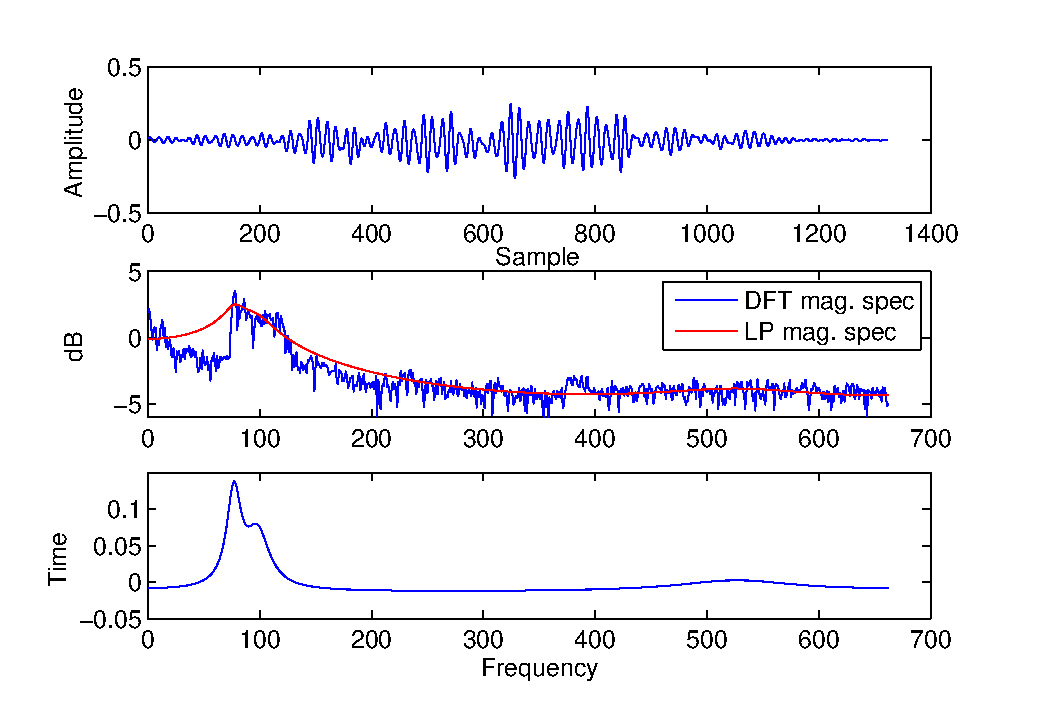
\includegraphics[width=0.5\textwidth,height=7cm]
{apgd.eps}
\caption{A frame of audio signal (top panel), corresponding LP
magnitude spectrum superimposed on DFT magnitude spectrum (middle panel) and
all-pole group delay function (bottom panel)  }
\label{fig:all-pole}
\end{figure}


Recently, feature vectors
derived from such a representation were used in speech \cite{drugman} and speaker
recognition \cite{padman}. 



%This is equivalent to a cascade of several
%first-order and second-order all-pole filters. The overall magnitude spectrum is
%the product of the individual magnitude spectra, and the overall phase spectrum
%is the sum of the individual phase spectra \cite{yegnaFormant}. Although
%developed for human speech, th






\section{Entropy-based segmentation of birdsong}

Computing the APGDF for every frame enables good time-frequency resolution of  the audio recording. Unlike the power spectrum, the APGDF can be negative. 
Since here we are interested only in the magnitudes and
locations of the frequency components, the sign of the APGDF is
ignored by taking the absolute value. Henceforth, APGDF means positive APGDF. 
 A sliding time-frequency window of width $w$ frames and frequency range
$fmin$ to $fmax$ is considered over the APGDF vectors. As in \cite{wang2013},
the entropy of this window is estimated using the expression
\begin{equation}
\label{eq:2}
h_{k}=-\sum_{n=kT+1}^{kT+w}\sum_{f=fmin}^{fmax} \uptau_N(n,f) \ln \uptau_N(n,f),
\end{equation}
where $T$ is the time-frequency window shift and $\uptau_N(n,f)$ is normalized APGDF. $\uptau_N(n,f)$ is estimated using the expression 
\begin{equation}
\uptau_N(n,f)=\frac {\uptau(n,f)}
{\sum_{n=kT+1}^{kT+w}\sum_{f=fmin}^{fmax} \uptau(n,f)},
\end{equation}

where $\uptau(n,f)$ is the positive APGDF at frame $n$ and frequency  \textit{f}.

The entropy calculated from time-frequency window is less susceptible to sudden changes in background as compared to the entropy calculated at each time instance \cite{wang2013}.The entropy of the time-frequency window containing bird call is lower than the one only containing the background. As the time-frequency window moves to the call region from background, the drop in entropy is observed. The entropy remains low if time-frequency window completely overlaps with the call period. The entropy increases as the window moves from call region to background. 

%The APGDF from figure
%\ref{fig:apgd} is shown in \ref{fig:apgdNoSign} after ignoring the sign.
%\begin{figure}[h]
%\centering
%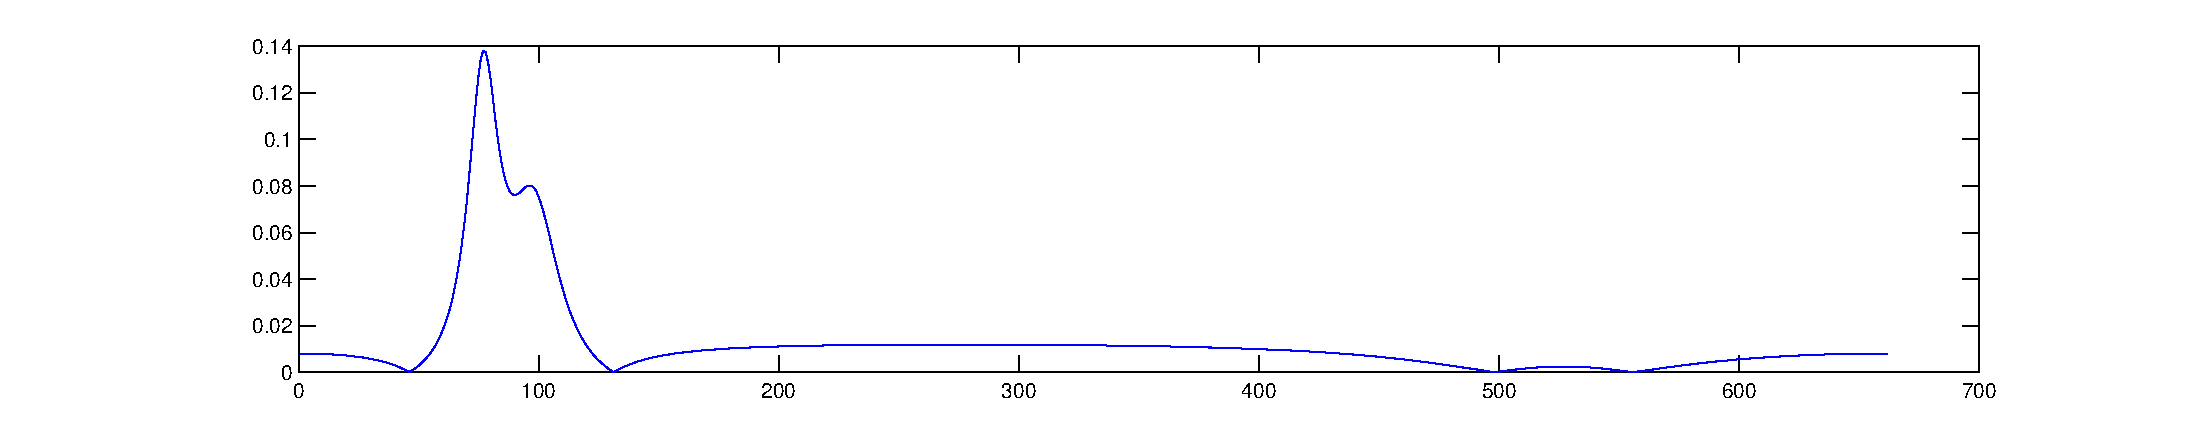
\includegraphics[width=0.5\textwidth,height=2cm]{apgdNoSign.eps}
%\caption{based on all pole model (in the bottom panel).}
%\label{fig:all-pole}
%\end{figure}



 


\subsection{Whitening APGDF before Entropy Calculation}

The drop in entropy during the presence of bird vocalizations makes it possible to detect call periods. Due to the presence of various background sounds e.g. rain, thunder, other animals etc., entropy of the background can  vary rapidly making it difficult to separate it from entropy  at a call period. To mitigate this problem to some extent, APGDF is whitened  before calculating entropy. The entropy calculated from whitened APGDF  is almost constant for background but dips enough to mark the presence of bird vocalizations. Due to this nature of background entropy, small change in entropy can be detected reliably.

To whiten the APGDF ($\uptau(n,f)$), the covariance matrix $C$ of the mean-subtracted
APGDF is estimated. The eigenvalue matrix $S$ and the eigenvector matrix
$U$ of $C$ are determined. The whitened APGDF
($\uptau_W(n,f)$) is calculated as:

\begin{equation}
\uptau_W(n,f)=\text{diag} \bigg(  \frac{1}{\sqrt{\text{diag(S)}+\epsilon}} \bigg )\times \text{U'} \times \uptau(n,f),
\end{equation}




Henceforth, the whitened APGDF is used to calculate entropy. The difference between entropy calculated from normal phase spectrum and whitened phase spectrum is evident in Figure \ref{fig:entropy}.

\begin{figure}[h]
\centering
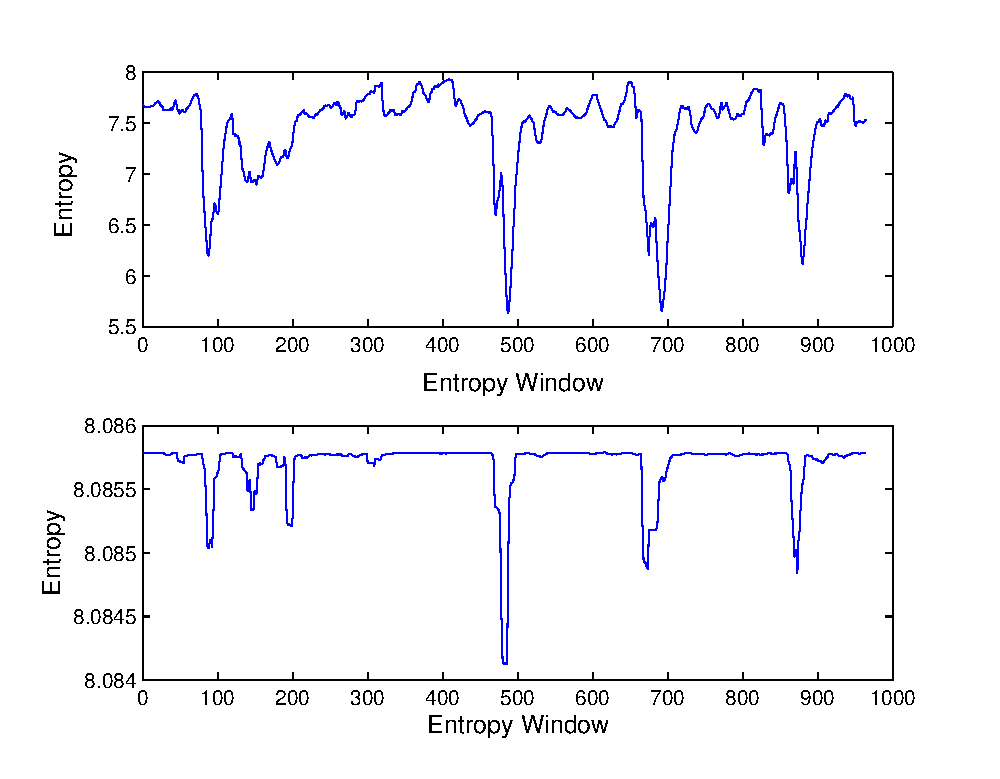
\includegraphics[width=0.5\textwidth,height=7.5cm]{Entropy_gd_white_non_white.eps}
\caption{ Entropy calculated from APGDF (Uppen Panel) and entropy calculated using white APGDF (Lower Panel).}
\label{fig:entropy}
\end{figure}



\subsection{Detecting change points using thresholding}



   
To detect the change points, extrema-based thresholding is used. Local minima and maxima are estimated on the entropy.  The thresholding is applied on the difference of  consecutive local maxima and local minima to determine the change point.  Two contiguous change points correspond to the start and end of a bird vocalization. These change points can be tracked back to get the start and end time of the vocalization in sound recording.     
   
   
   




\section{Experimentation and Performance Analysis}


The proposed algorithm is evaluated on two datasets. The first consists of recordings of a single species, the Cassin's vireo,
and second is a subset of the MLSP 2013 bird classification challenge, consisting of recordings from several species. In
the Cassin's vireo dataset \cite{data1}, the total duration of recordings
is about 45 minutes, out of which about 5 minutes correspond
to the calls. These recordings are fairly clean and have less
background noise. Phrase annotations are provided with the dataset. The start and end of these annotations are used as the ground truth. 

The MLSP 2013 dataset \cite{data2} is much nosier and includes
wind and rain in the background.The dataset is collected in the H. J. Andrews (HJA) long-term experimental research forest in Oregon.
The recordings are done for over two years at 13 different locations. Twenty Five files of ten seconds length are taken from the data to evaluate the proposed method. Manual annotations are done to mark the presence of bird vocalizations in these audio files.  


The proposed algorithm is compared with a modified version of technique proposed in \cite{wang2013}. The entropy estimated from whitened power spectrum is used to determine the change points. Similar to the proposed algorithm, extrema-based thresholding is referred to determine the change points. Thus, entropy from power spectrum is compared to the entropy from APGDF.
 
The frame length of 20 ms and increment of  
5 ms is used to divide the audio signal into the frames. For each frame, APGDF vector is calculated.
The whitening is applied to APGDF before calculating entropy.
A time-frequency window of length
$w$=138.8 ms is used along with increment of $T$ = 15 ms to estimate the
entropy (see equation \ref{eq:2}).  The frequency range of the time-frequency window is set from $f_{min}$=1.5 kHz to $f_{max}$=7 kHz \cite{wang2013}.  

Receiver operating characteristic (ROC) curves are used to analyze the performance of both the techniques. True positive rate and false alarm rate are calculated using following equations:

\begin{equation}
\text{TPR} (\%)=\frac{\text{Correctly Classified Call Frames}} {\text{Total Call Frames}} \times 100 
\end{equation}




\begin{equation}
\text{FAR} (\%)=\frac{\text{Wrongly Classified As Call Frames}} {\text{Total Background Frames}} \times 100 
\end{equation}



 Figure \ref{fig:ROCdata1} depicts ROC curves comparing performance of the methods based on power spectrum and APGDF on Cassin's Vireo dataset. It is clear from  figure \ref{fig:ROCdata1} that the APGDF method outperforms the power spectrum method.

\begin{figure}[h]
\centering
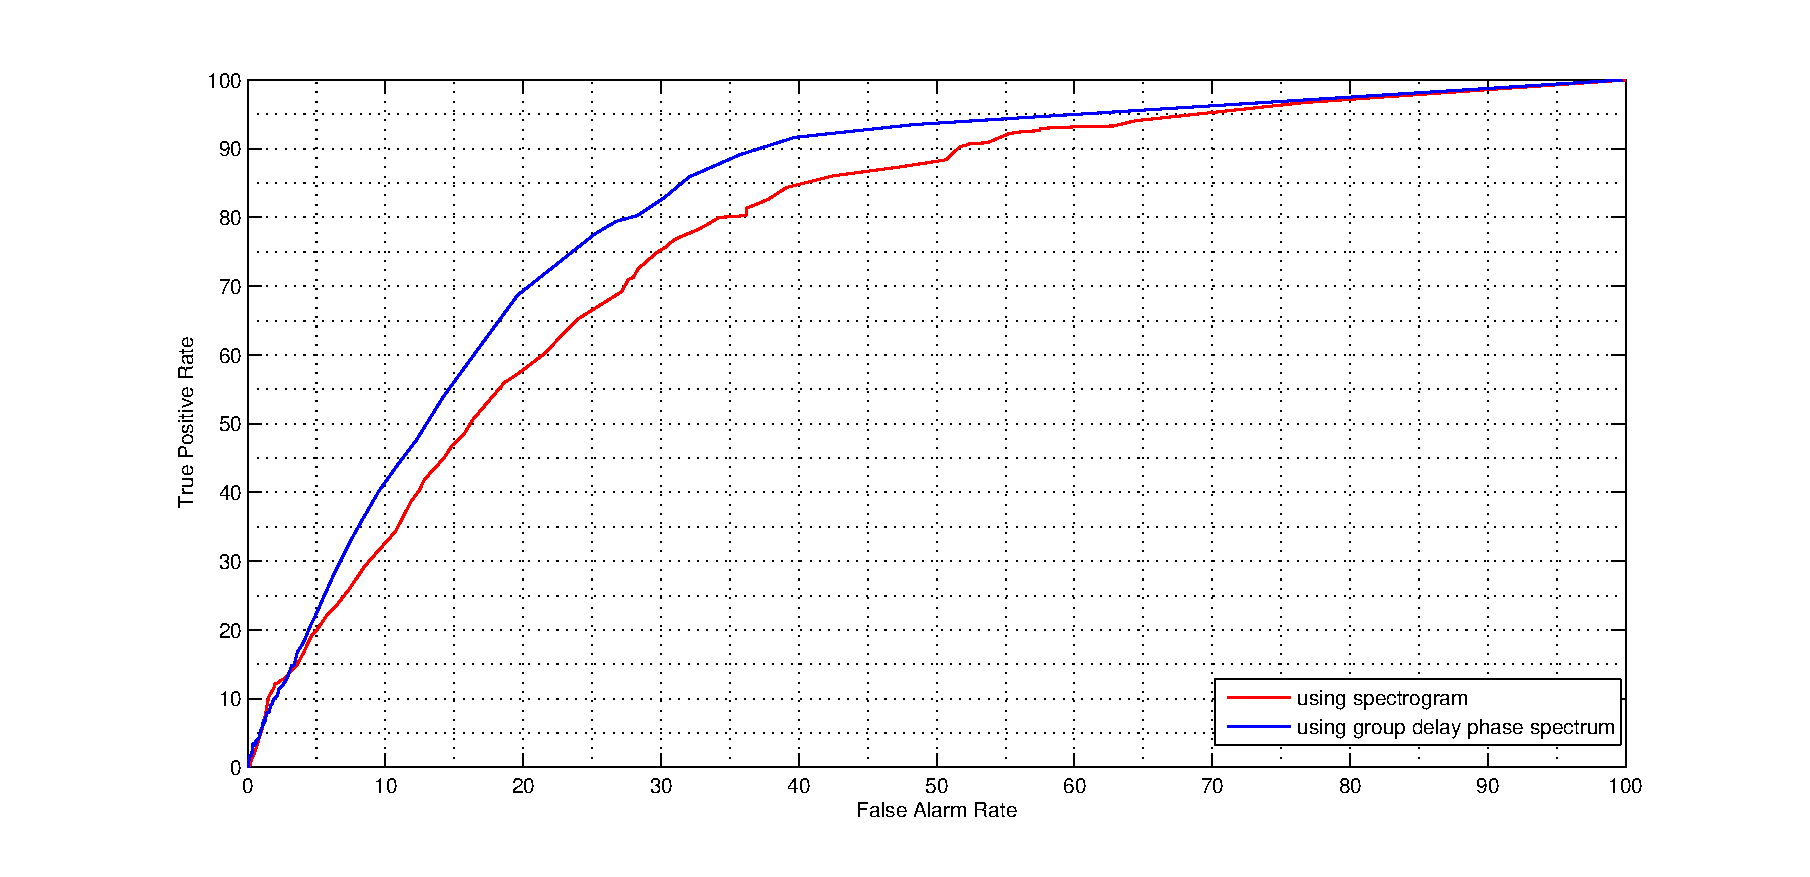
\includegraphics[width=0.5\textwidth,height=7cm]{ROC_gr_delay_5_VS_spectrogram.eps}
\caption{ROC  curves  comparing  performance  of  methods based on APGDF and spectrogram on Cassin's Vireo dataset.}
\label{fig:ROCdata1}
\end{figure}



 
 
 
 Figure \ref{fig:ROCdata2} shows ROC curves comparing performance of methods based on entropy calculated from APDGF  and spectrogram on MLSP dataset. Here too, APGDF based method outperforms spectrogram based method for almost all the operating points. 

 
\begin{figure}[!ht]
	\centering
	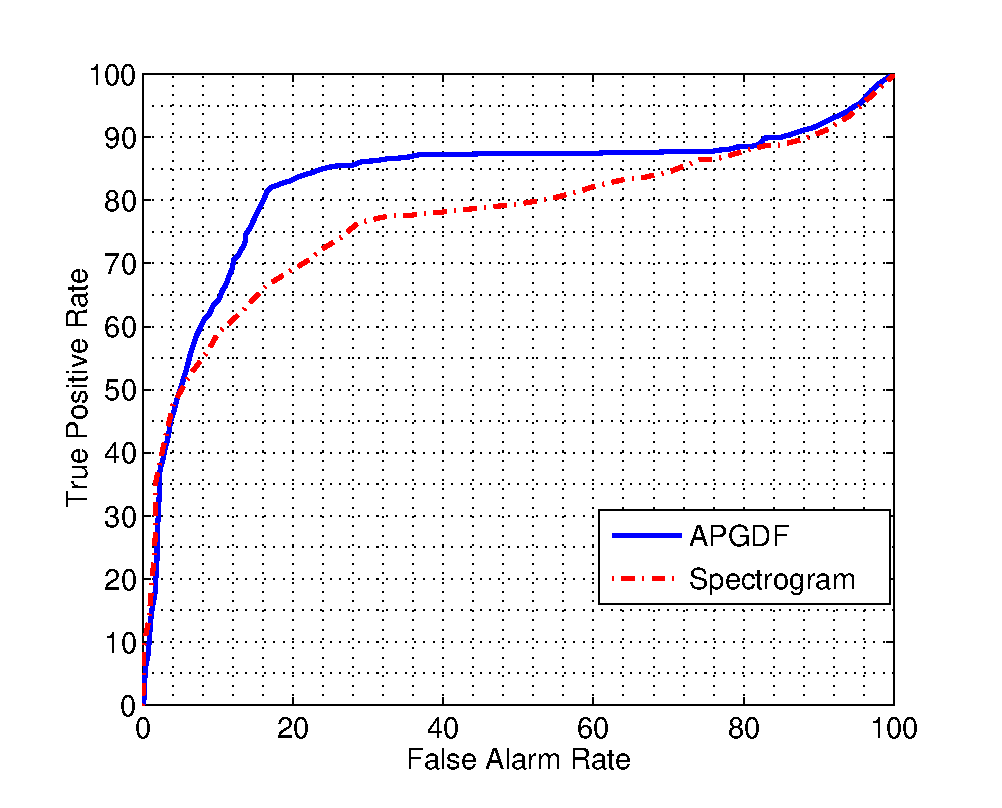
\includegraphics[width=0.5\textwidth,height=7cm] {ROC_gr_delay_10_VS_spectrogram_data2.eps}
	\caption{ROC curves comparing performance of methods based on APGDF and spectrogram on MLSP dataset }   
	\label{fig:ROCdata2}
\end{figure} 




 \subsection{Model Order  vs AIC}
 
 
 To establish the optimum model order, Akaike Information criteria (AIC)  \cite{makhoul} is used. Figure \ref{fig:AIC_cassins} depicts the AIC for different model orders for Cassin's Vireo phrases.  
 
 
 \begin{figure}[!ht]
	\centering
	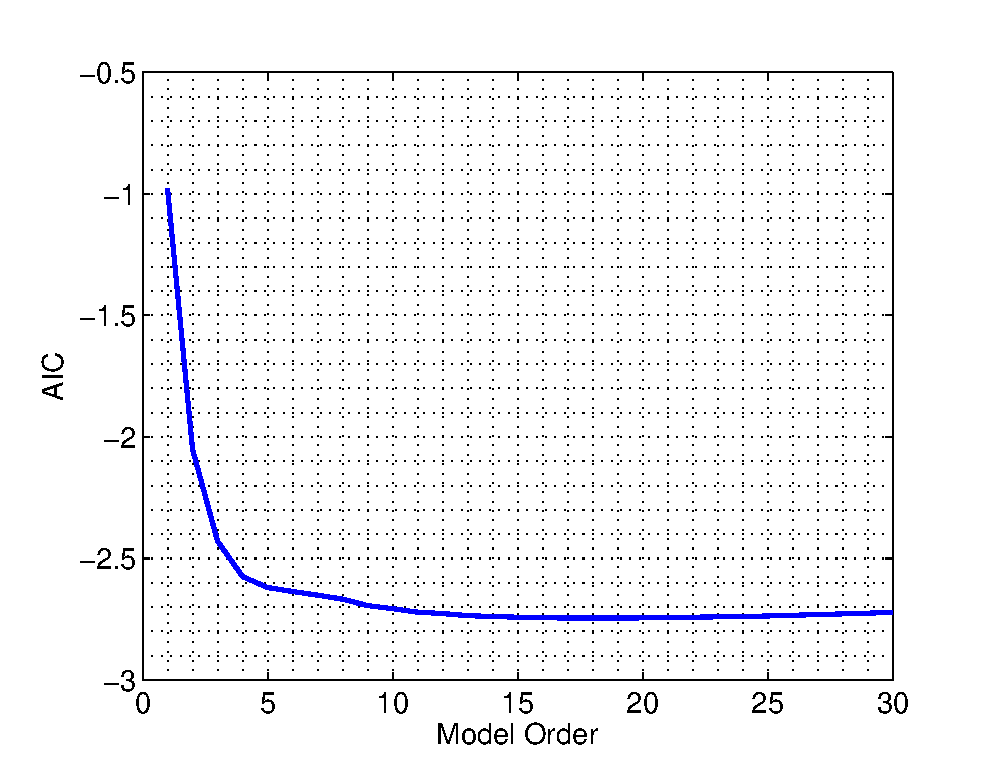
\includegraphics[width=0.5\textwidth,height=6cm] {cassins_AIC.eps}
	\caption{AIC vs model order for Cassin's Vireo }   
	\label{fig:AIC_cassins}
\end{figure} 

 
 
Figure \ref{fig:AIC_3} depicts the AIC for different model orders for three different bird species i.e. Cuckoo, Great Barbet and Laughing Thresh. 

 \begin{figure}[!ht]
	\centering
	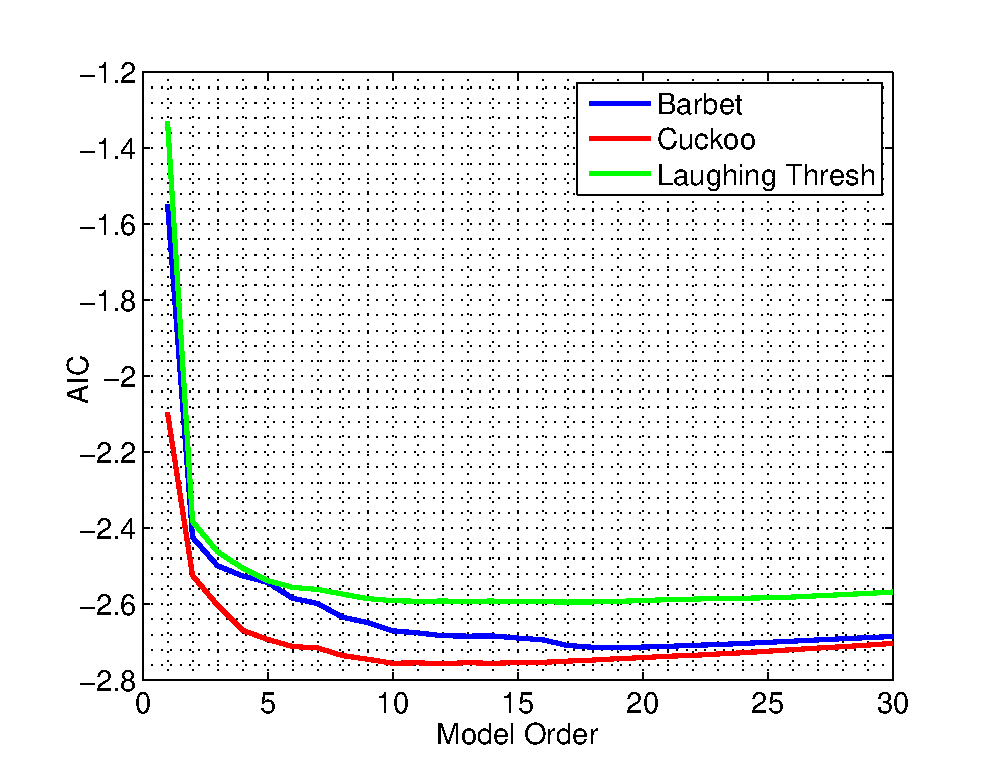
\includegraphics[width=0.5\textwidth,height=7 cm] {model_order_vs_AIC.eps}
	\caption{AIC vs model order for three different species }   
	\label{fig:AIC_3}
\end{figure} 


 
 
 



%%  write formullae for calculating correct, missed detection and false alarms
\begin{comment}
Table 1 shows results generated by applying entropy based segmentation with thresholding on different sound recordings. 

  



\begin{table}[]
	\centering
	\caption{Table showing Correct (\%) Missed Detection(\%) and False alarm (\%) for particular thresholds and moving average windows } 
	\label{Table 1}

	\begin{tabular}{|c|c|c|c|c|c|}
		\hline
		\textbf{File} & \textbf{Span} & \textbf{Threshold} & \textbf{Correct (\%)} & \textbf{False Alarm (\%)} & \textbf{Missed Detection (\%)} \\ \hline
		1.wav         & 9             & 1.2                & 77.7                  & 15.6                      & 60.5                           \\
	\hline	2.wav         & 3             & 1.45               & 73                    & 45                        & 25                             \\
		\hline	3.wav         & 3             & 1.5                & 71                    & 22                        & 54                             \\
		\hline	4.wav         & 9             & 1.15               & 75.1              & 21                  & 51.5                       \\
		\hline	5.wav         & 7             & 1.5                & 76.5                  & 18.5                      & 45                             \\
	\hline		6.wav         & 9             & 1.25               & 82.1              & 15.07                  & 32.2                       \\
		\hline	7.wav         & 7             & 1.25               & 79.6              & 17.8                  & 46.7                       \\
		\hline	8.wav         & 9             & 1.15               & 78.8              & 19.3                  & 35.1                      \\
		\hline	9.wav         & 5             & 1.5                & 86.06              & 13.6                  & 17.9                       \\
	\hline		10.wav        & 9             & 1.6                & 79.6              & 18.3                  & 28.31                       \\
		\hline	11.wav        & 3             & 1.45               & 91.1                  & 32.7                      & 7.53                           \\
		\hline	12.wav        & 7             & 1.4                & 85.1              & 11.3                   & 38.1      \\ \hline               	
	 
	\end{tabular}

\end{table}

\end{comment}
 
 
\section{Conclusion}
We propose an entropy based bird vocalization segmentation method where entropy is calculated from Group Delay phase spectrum. It is also established that whitening the power or phase spectrum before entropy calculation improves the performance of entropy based segmentation. From experimentation,it is clear that the proposed group delay based method outperforms the power spectrum based method.  



  \newpage
  \eightpt
  \bibliographystyle{IEEEtran}

  \bibliography{mybib}

%  \begin{thebibliography}{9}
%    \bibitem[1]{Davis80-COP}
%      S.\ B.\ Davis and P.\ Mermelstein,
%      ``Comparison of parametric representation for monosyllabic word recognition in continuously spoken sentences,''
%      \textit{IEEE Transactions on Acoustics, Speech and Signal Processing}, vol.~28, no.~4, pp.~357--366, 1980.
%    \bibitem[2]{Rabiner89-ATO}
%      L.\ R.\ Rabiner,
%      ``A tutorial on hidden Markov models and selected applications in speech recognition,''
%      \textit{Proceedings of the IEEE}, vol.~77, no.~2, pp.~257-286, 1989.
%    \bibitem[3]{Hastie09-TEO}
%      T.\ Hastie, R.\ Tibshirani, and J.\ Friedman,
%      \textit{The Elements of Statistical Learning -- Data Mining, Inference, and Prediction}.
%      New York: Springer, 2009.
%    \bibitem[4]{YourName16-XXX}
%      F.\ Lastname1, F.\ Lastname2, and F.\ Lastname3,
%      ``Title of your INTERSPEECH 2016 publication,''
%      in \textit{Interspeech 2016 -- 16\textsuperscript{th} Annual Conference of the International Speech Communication Association, September 8–12, San Francisco, California, USA, Proceedings, Proceedings}, 2016, pp.~100--104.
%  \end{thebibliography}

\end{document}
